\thispagestyle{diendandayvahoctoannone}
\pagestyle{diendandayvahoctoan}
\everymath{\color{diendantoanhoc}}
\graphicspath{{../diendantoanhoc/pic/}}
\blfootnote{$^{1}$\color[named]{diendantoanhoc}Trường Liên cấp Hội nhập Quốc tế iSchool Quảng Trị.}
\begingroup
\AddToShipoutPicture*{\put(0,616){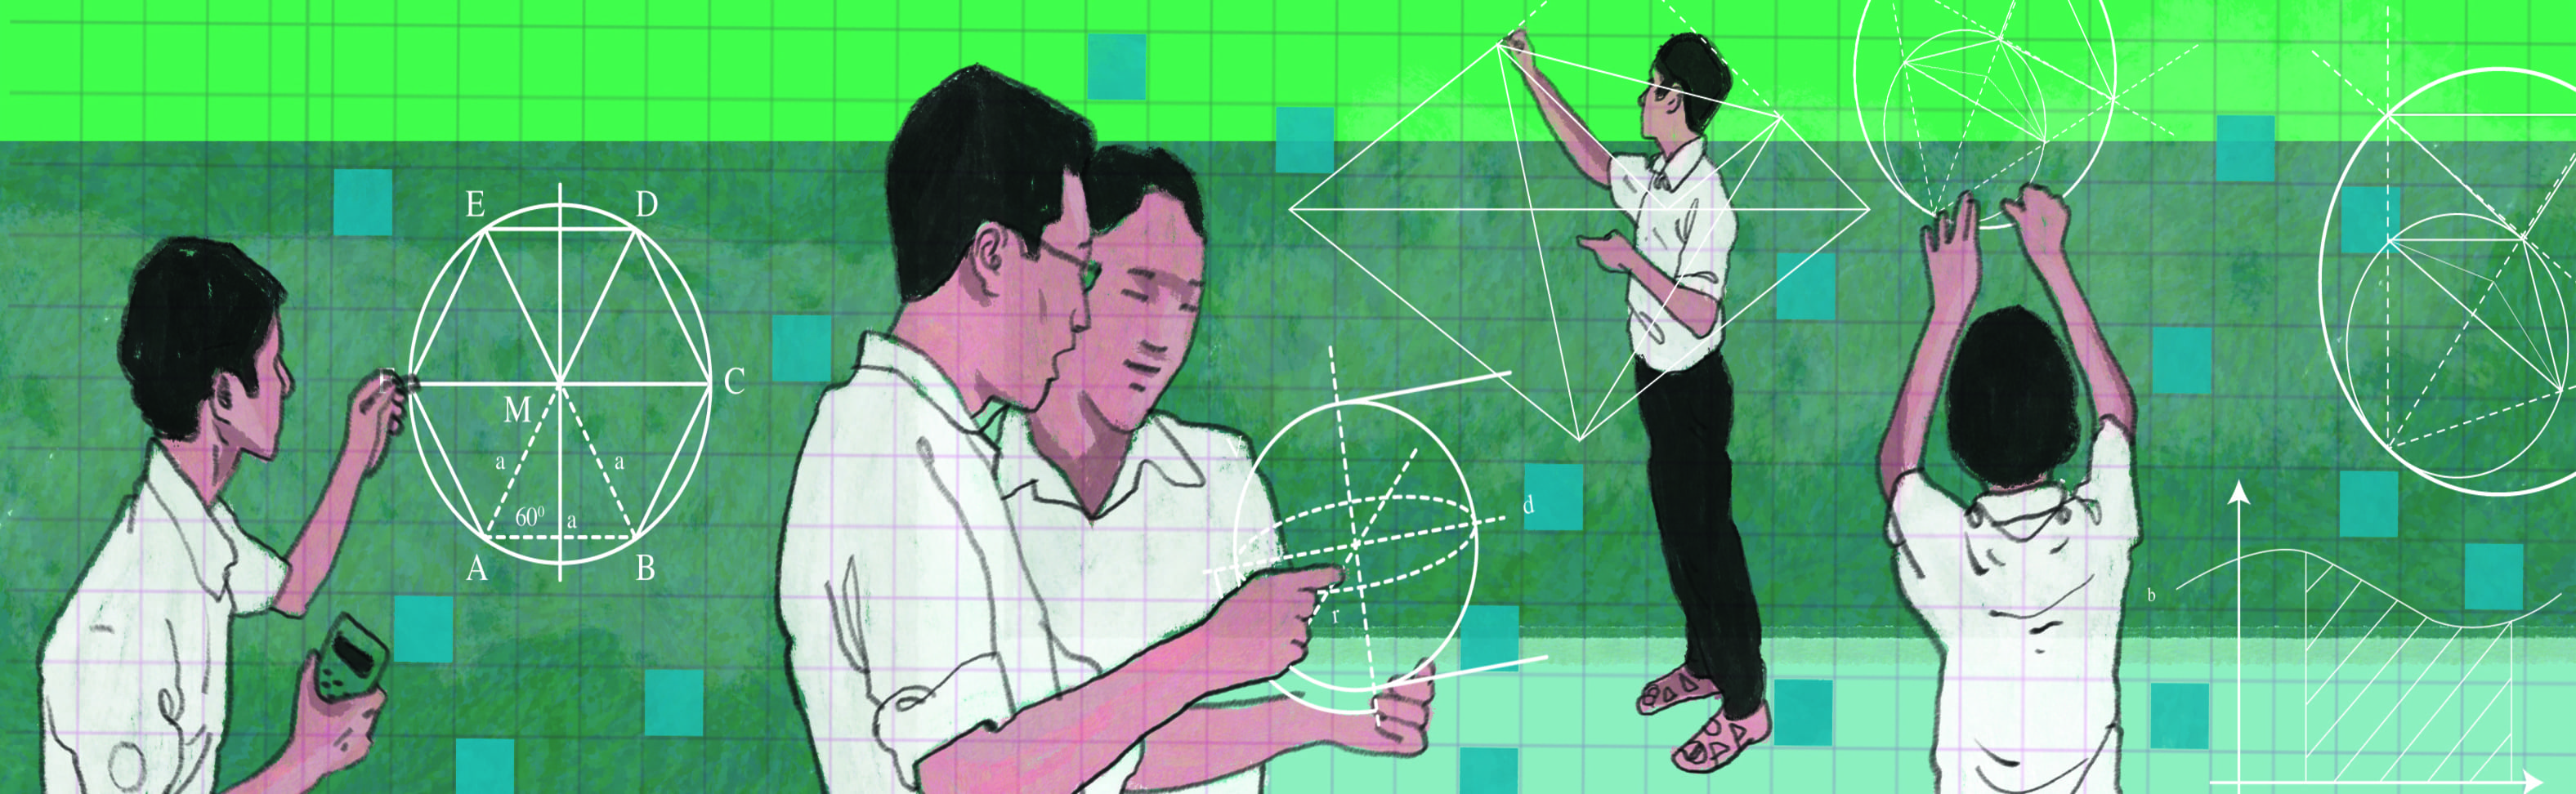
\includegraphics[width=19.3cm]{../bannerdiendan}}}
\AddToShipoutPicture*{\put(114,555){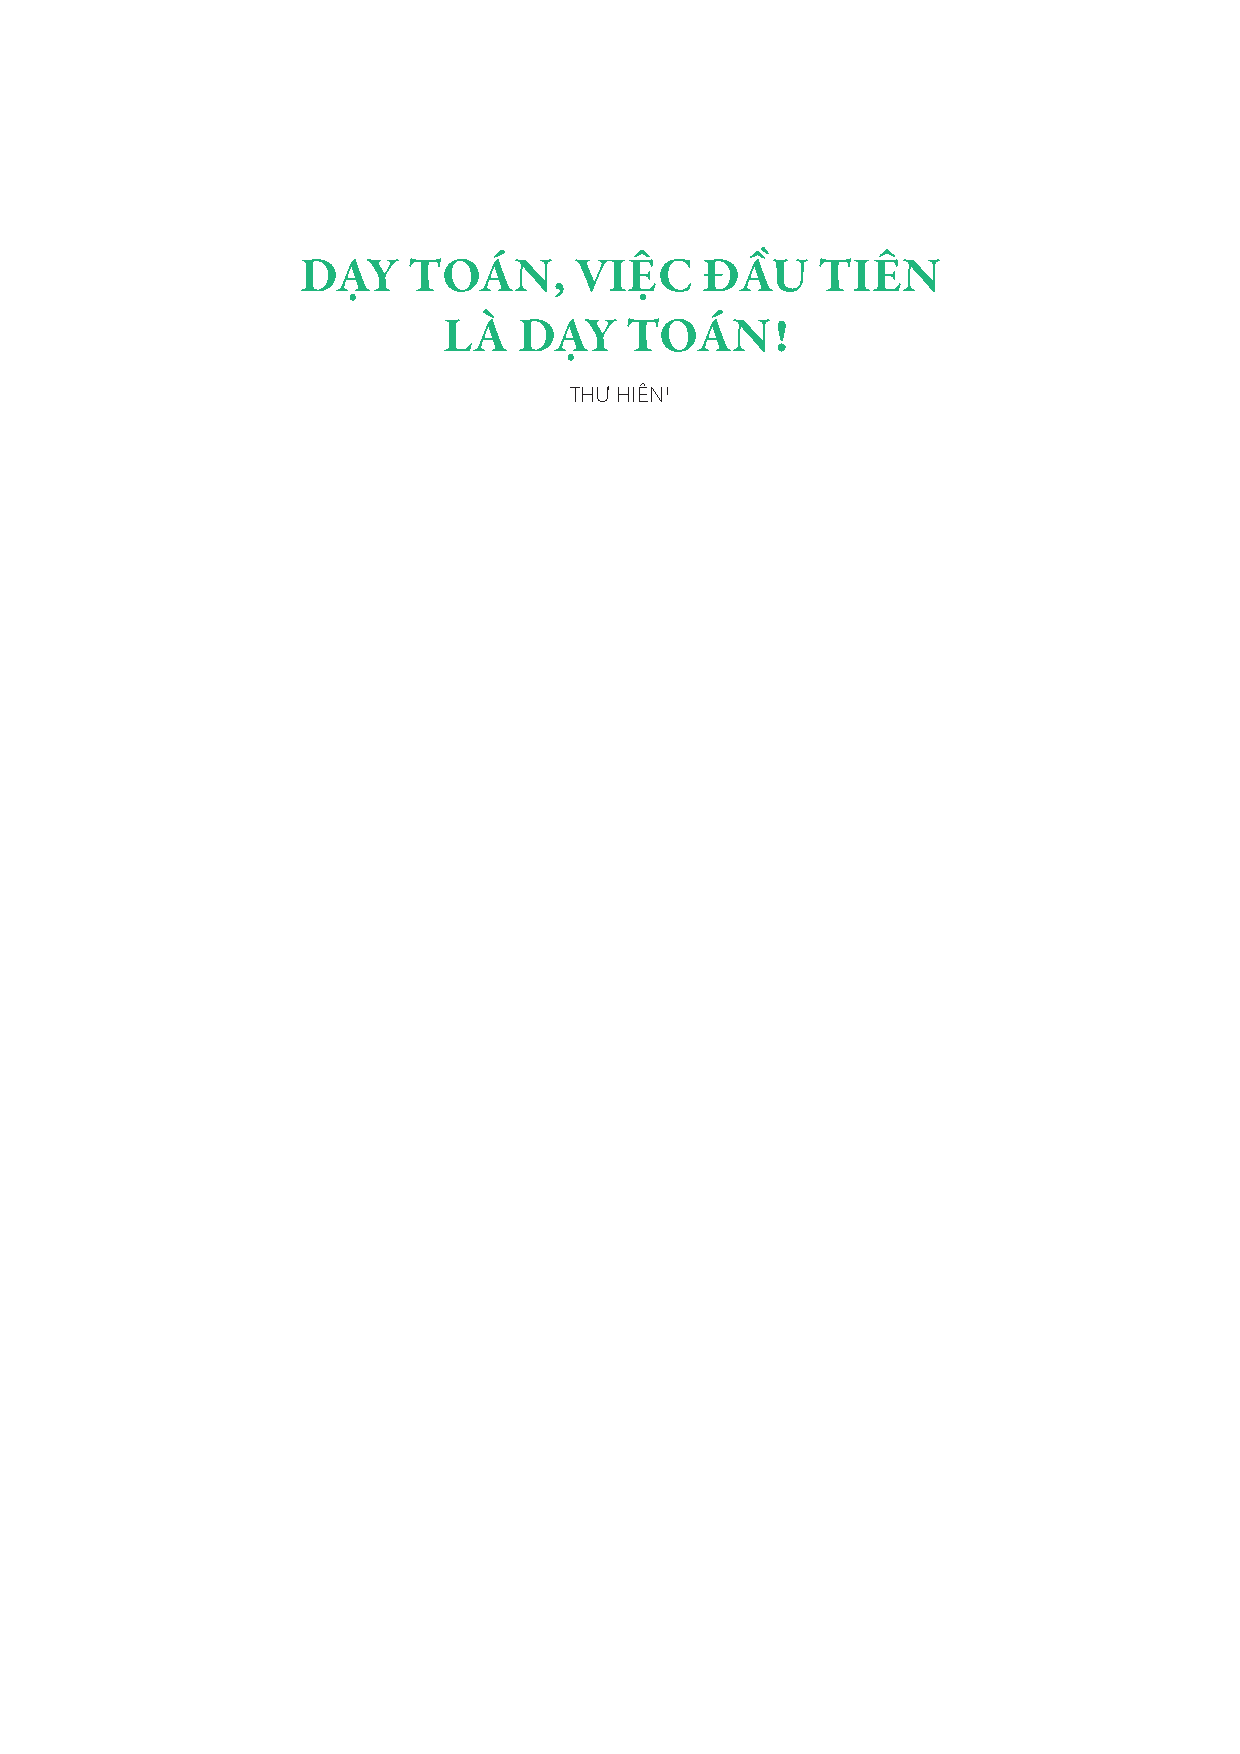
\includegraphics[scale=1]{../tieude.pdf}}}
\centering
\endgroup
\vspace*{162pt}

	\textit{\textbf{\color{diendantoanhoc}LTS.} Góp phần nâng cao chất lượng giảng dạy Chương trình Toán phổ thông mới, Tòa soạn xin giới thiệu chia sẻ của cô giáo Nguyễn Thụy Việt Anh về một số ý tưởng trong việc dạy bài Hình có trục đối xứng, môn Toán lớp $6$. Chúng tôi mong tiếp tục nhận được nhiều chia sẻ từ các thầy \linebreak cô giáo.}
\begin{multicols}{2}
	\textbf{\color{diendantoanhoc}Mục tiêu.} Về kiến thức:  Nhận biết được hình có trục đối xứng; trục đối xứng của các hình hình học đơn giản.  Về năng lực: Biết được trục đối xứng của một hình trên giấy bằng cách gấp đôi tờ giấy; cách gấp giấy để cắt chữ hoặc một số hình đơn giản có trục đối xứng. Về phẩm chất: Bồi dưỡng trí tưởng tượng, hứng thú học tập, ý thức làm việc nhóm, ý thức tìm tòi, khám phá và sáng tạo cho học sinh.
	\vskip 0.1cm
	\textbf{\color{diendantoanhoc}Thiết bị dạy học và học liệu.} Đối với giáo viên: Một số bức hình có trục đối xứng hoặc đồ vật hay biểu tượng có trục đối xứng, một số mẫu chữ cái hoặc số có trục đối xứng, giấy màu hoặc bìa cứng, kéo và máy tính (nếu có). Đối với học sinh: Giấy màu hoặc bìa cứng, kéo.
	\vskip 0.1cm
	\textbf{\color{diendantoanhoc}Tiến trình dạy học.}
	\vskip 0.1cm  
	$\pmb{1.}$ \textbf{\color{diendantoanhoc}Mở đầu}
	\vskip 0.1cm
	\textit{Mục tiêu:} Tạo tình huống vào bài học từ hình ảnh thực tế, ứng dụng thực tế từ các hình trong bài; học sinh hình dung được một cách sơ khai về dạng hình ảnh của một hình trong tự nhiên có trục đối xứng.
	\vskip 0.1cm
	\textit{Thực hiện:} Giáo viên chiếu hình ảnh hoặc video của một số hình ảnh có tính đối xứng trục. (Giáo viên có thể vạch đường kẻ dọc cho học sinh nhận xét nửa bên trái và nửa bên phải của hình; đối với mặt hồ thì nhận xét phía trên mặt hồ và bóng phía dưới nước). 
	\begin{figure}[H]
		\vspace*{-5pt}
		\centering
		\captionsetup{labelformat= empty, justification=centering}
		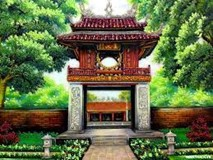
\includegraphics[height=0.37\linewidth]{1}
		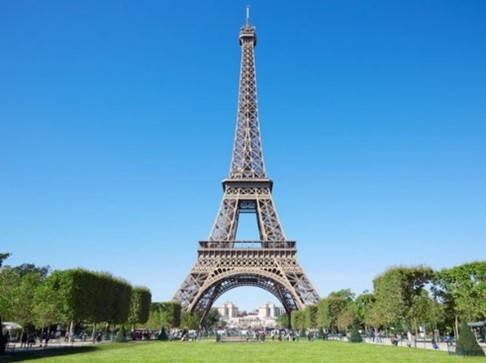
\includegraphics[height=0.37\linewidth]{2}
		\caption{\small\textit{\color{diendantoanhoc}Khuê Văn Các \hspace*{45pt} Tháp Eiffel.}}
		
		\vspace*{2pt}
		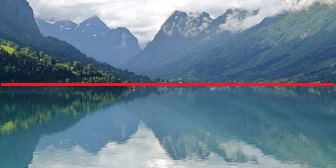
\includegraphics[width= 1\linewidth]{3}
		\caption{\small\textit{\color{diendantoanhoc}Mặt hồ.}}
		\vspace*{-10pt}
	\end{figure}
	Lớp thảo luận về nhận định:  ``Trong cuộc sống, chúng ta hay gặp rất nhiều hình ảnh đẹp. Nếu như các em để ý một chút thì sẽ thấy rằng các hình ảnh đều có sự cân đối, hài hòa". 
	\vskip 0.1cm
	Đặt vấn đề: Điều gì đã đem lại sự cân đối, hài hòa đó?
	\vskip 0.1cm
	Giáo viên giới thiệu qua nội dung bài học:
	\vskip 0.1cm
	$\bullet$	Nhận biết hình có trục đối xứng và hình có tâm đối xứng.
	\vskip 0.1cm
	$\bullet$	Nhận biết trục đối xứng và tâm đối xứng của một số hình đơn giản.
	\vskip 0.1cm
	$\bullet$	Gấp giấy để cắt được một số hình có trục đối xứng hoặc tâm đối xứng đơn giản.
	\vskip 0.1cm
	$\pmb{2.}$ \textbf{\color{diendantoanhoc}Hình thành kiến thức mới}
	\vskip 0.1cm
	${2.1}$ \textit{Hình có trục đối xứng trong thực tế}
	\vskip 0.1cm
	\textit{Mục tiêu:} Học sinh trình bày được khái niệm và nhận biết được hình có trục đối xứng và trục đối xứng của một hình, tìm được ví dụ thực tế về hình có trục đối xứng để biết được một số ứng dụng tính đối xứng của hình trong đời sống.
	\vskip 0.1cm
	\textit{Thực hiện:} Giáo viên giới thiệu một số thao tác để minh họa tính đối xứng trục, ví dụ:
	\vskip 0.1cm
	$\bullet$   Mở video có hình con bướm ở trong tự nhiên và đặt câu hỏi về hai cánh của con bướm; 
	\vskip 0.1cm
	$\bullet$	Gấp đôi hình tròn theo một đường thẳng đi qua tâm và yêu cầu nhận xét về hai nửa hình tròn sau khi gấp;
	\vskip 0.1cm
	$\bullet$	Gấp đôi một tờ giấy A$4$, rồi dùng kéo cắt một đường sau đó mở ra.
	Từ đó giáo viên đi đến khái niệm: ``Nếu có một đường thẳng chia một hình thành hai phần mà khi gấp hình theo đường thẳng đó, ta thấy hai phần chồng khít lên nhau thì hình đó là hình có trục đối xứng và đường thẳng nói trên là trục đối xứng của hình."
	\vskip 0.1cm
	\textit{Trò chơi ``Ai nhanh hơn?"}
	\vskip 0.1cm
	Giáo viên chuẩn bị trước ở nhà những tấm thẻ có các chữ cái $A, B, C,\ldots$ Chia lớp thành $2$ đội hoặc $3$ đội (tùy vào số lượng học sinh mỗi lớp). Trong vòng $1$ phút, đội nào gắn được nhiều hơn và nhanh hơn những tấm thẻ có các chữ cái có trục đối xứng lên bảng sẽ là đội chiến thắng.
	\vskip 0.1cm
	\begin{figure}[H]
		\vspace*{-5pt}
		\centering
		\captionsetup{labelformat= empty, justification=centering}
		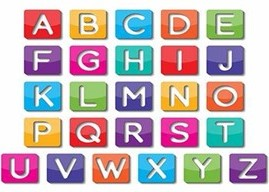
\includegraphics[width= 1\linewidth]{4}
		\caption{\small\textit{\color{diendantoanhoc}Hình ảnh các chữ cái (Ảnh: Internet).}}
		\vspace*{-10pt}
	\end{figure}
	$2.2$ \textit{Trục đối xứng của một số hình phẳng}
	\vskip 0.1cm
	\textit{Mục tiêu:} Nhận biết được trục đối xứng của hình tròn, hình thoi, hình chữ nhật. Biết được số trục đối xứng của các hình trên. Gấp giấy để tìm trục đối xứng của đoạn thẳng, hình tam giác đều, hình vuông, hình lục giác đều. Học sinh biết được một hình có thể có nhiều hoặc thậm chí là vô số trục đối xứng. Biết cách gấp giấy để cắt được các chữ có trục đối xứng đơn giản. Hình dung được toàn bộ một hình có trục đối xứng khi chỉ được biết một nửa hình đó. Hình dung được trục đối xứng của một hình thông qua sự đối xứng của các chi tiết.
	\vskip 0.1cm
	\textit{Thực hiện:} chia thành nhóm và phát cho mỗi nhóm một tờ giấy A$0$ để làm các nội dung sau:
	\vskip 0.1cm
	$\bullet$	Vẽ một đường tròn trên giấy rồi cắt theo nét vẽ ta được một hình tròn. Gấp đôi hình tròn đó theo một đường thẳng đi qua tâm. Em hãy cho biết trục đối xứng của hình tròn là đường thẳng nào?
	\vskip 0.1cm
	$\bullet$	Cắt một hình thoi bằng giấy. Hãy tìm trục đối xứng của nó bằng cách gấp giấy. Trục đối xứng của nó là đường thẳng nào? Em tìm được mấy trục đối xứng?
	\vskip 0.1cm
	$\bullet$	Vẽ rồi cắt một hình chữ nhật bằng giấy. Hãy tìm trục đối xứng của nó bằng cách gấp giấy. Trục đối xứng của nó là đường thẳng nào? Em tìm được mấy trục đối xứng?
	\vskip 0.1cm
	\textit{Thảo luận theo phương  thức ``khăn trải bàn"}
	\vskip 0.1cm 
	Trên giấy A$0$ chia thành các phần, gồm phần chính giữa và các phần xung quanh được chia theo số thành viên của nhóm (ví dụ nhóm $4$ người). Mỗi người ngồi vào vị trí tương ứng với từng phần xung quanh.
	\begin{figure}[H]
		\vspace*{-5pt}
		\centering
		\captionsetup{labelformat= empty, justification=centering}
		\begin{tikzpicture}[diendantoanhoc,scale=0.88,node font = \small]
			\draw  (0.,2.)-- (0.,0.);
			\draw  (0.,0.)-- (4.,0.);
			\draw  (4.,0.)-- (4.,2.);
			\draw  (4.,2.)-- (0.,2.);
			\draw  (4.,2.)-- (6.,4.);
			\draw  (6.,4.)-- (-2.,4.);
			\draw  (-2.,4.)-- (-2.,-2.);
			\draw  (-2.,-2.)-- (6.,-2.);
			\draw  (6.,-2.)-- (6.,4.);
			\draw  (4.,0.)-- (6.,-2.);
			\draw  (0.,0.)-- (-2.,-2.);
			\draw  (0.,2.)-- (-2.,4.);
			\draw  (1.5925909332759858,2.200395216725359)-- (2.4062492999758063,2.200395216725359);
			\draw  (2.4062492999758063,2.200395216725359)-- (2.4062492999758063,3.014053583425179);
			\draw  (2.4062492999758063,3.014053583425179)-- (1.592590933275986,3.0140535834251794);
			\draw  (1.592590933275986,3.0140535834251794)-- (1.5925909332759858,2.200395216725359);
			\draw  (4.2094921667159495,0.6060646333270615)-- (5.0011597667482075,0.5950692499932801);
			\draw  (5.0011597667482075,0.5950692499932801)-- (5.0121551500819885,1.3867368500255381);
			\draw  (5.0121551500819885,1.3867368500255381)-- (4.2204875500497305,1.3977322333593194);
			\draw  (4.2204875500497305,1.3977322333593194)-- (4.2094921667159495,0.6060646333270615);
			\draw  (1.603586316609767,-0.9992613334050172)-- (2.4062492999758063,-0.9882659500712359);
			\draw  (2.4062492999758063,-0.9882659500712359)-- (2.3952539166420252,-0.185602966705197);
			\draw  (2.3952539166420252,-0.185602966705197)-- (1.592590933275986,-0.19659835003897802);
			\draw  (1.592590933275986,-0.19659835003897802)-- (1.603586316609767,-0.9992613334050172);
			\draw  (-1,0.6)-- (-0.2,0.6);
			\draw  (-0.2,0.6)-- (-0.2,1.4);
			\draw  (-0.2,1.4)-- (-1.0,1.4);
			\draw  (-1.0,1.4)-- (-1,0.6);
			\draw (2,1) node[align = center] {\textbf{Ý kiến chung} \\ \textbf{của cả nhóm}};
			\draw (2,-1.5) node {Viết ý kiến cá nhân};
			\draw (2,3.5) node {Viết ý kiến cá nhân};
			\draw (5.5,1) node[rotate = -90] {Viết ý kiến cá nhân};
			\draw (-1.5,1) node[rotate = 90] {Viết ý kiến cá nhân};
			\draw (2,-0.6) node {$3$};
			\draw (2,2.6) node {$1$};
			\draw (4.6,1) node {$2$};
			\draw (-0.6,1) node {$4$};
		\end{tikzpicture}
		\caption{\small\textit{\color{diendantoanhoc}Sơ đồ kỹ thuật ``Khăn trải bàn".}}
		\vspace*{-5pt}
	\end{figure}
	Mỗi cá nhân làm việc độc lập trong khoảng vài phút, tập trung suy nghĩ để làm bài tập theo cách nghĩ, cách hiểu riêng của mỗi cá nhân và viết vào phần giấy của mình trên tờ A$0$. Trên cơ sở ý kiến của mỗi cá nhân, học sinh thảo luận nhóm, thống nhất ý kiến và viết vào phần chính giữa của tờ giấy A$0$ ``khăn trải bàn".
	\vskip 0.1cm
	Trong trường hợp số học sinh trong nhóm quá đông, không đủ chỗ trên ``khăn trải bàn", giáo viên có thể phát cho học sinh các mảnh giấy nhỏ để học sinh ghi ý kiến cá nhân, sau đó đính vào phần xung quanh ``khăn trải bàn". Những ý kiến trùng nhau có thể đính chồng lên nhau. Những ý kiến không thống nhất, cá nhân có quyền bảo lưu và được giữ lại ở phần xung quanh của ``khăn trải bàn".
	\vskip 0.1cm
	Học sinh thảo luận nhóm và trình bày kết quả theo kỹ thuật ``Khăn trải bàn", giáo viên phân tích, dẫn dắt, cho học sinh rút ra nhận xét.  
		\begin{figure}[H]
		\vspace*{-5pt}
		\centering
		\captionsetup{labelformat= empty, justification=centering}
		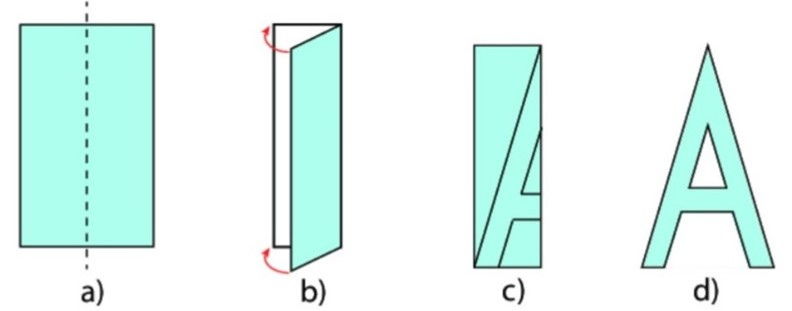
\includegraphics[width= 1\linewidth]{6}
		%		\caption{\small\textit{\color{}.}}
%		\vspace*{-10pt}
	\end{figure}
	\textit{Cắt chữ:} Giáo viên hướng dẫn và làm mẫu cắt chữ A theo các bước:
	\vskip 0.1cm
	Thực hiện tương tự với các chữ E, T. 
	\vskip 0.1cm
	$\pmb{3.}$ \textbf{\color{diendantoanhoc}Củng cố}
	\vskip 0.1cm
	Giáo viên  nhắc lại kiến thức bài học bằng sơ đồ tư duy để khắc sâu kiến thức.
	\begin{figure}[H]
		\vspace*{-5pt}
		\centering
		\captionsetup{labelformat= empty, justification=centering}
		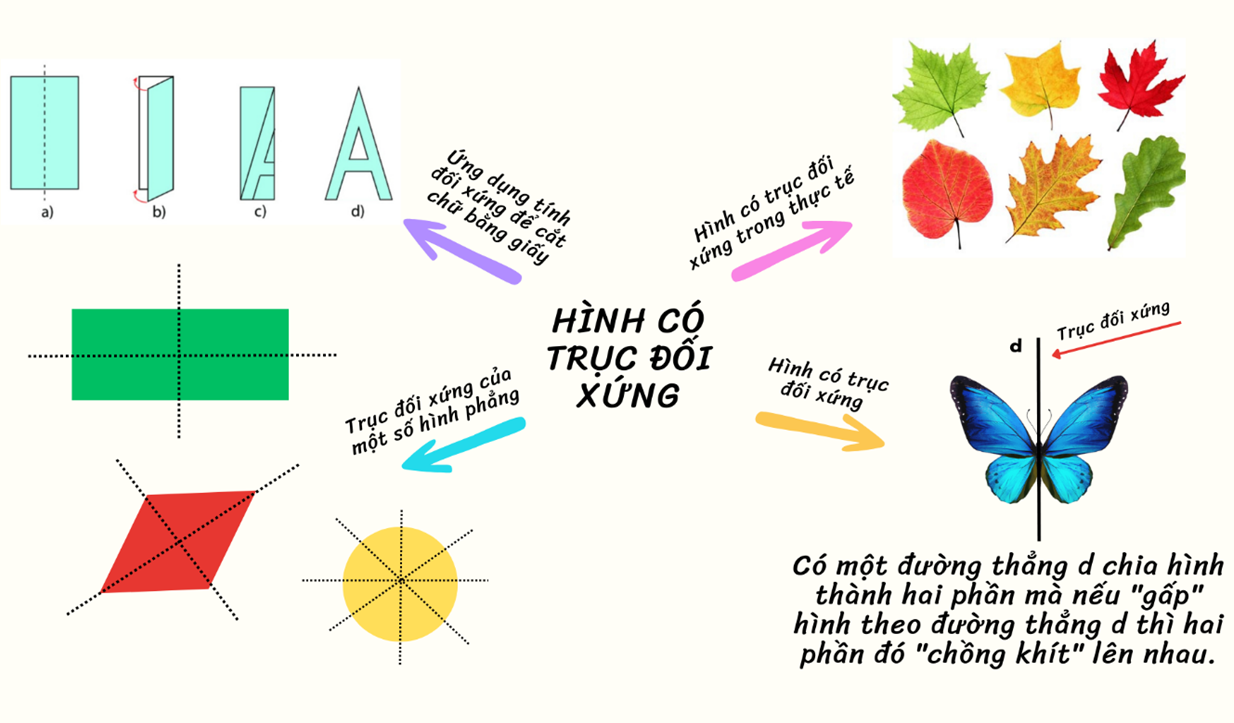
\includegraphics[width= 1\linewidth]{7}
		\caption{\small\textit{\color{diendantoanhoc}Sử dụng Canva để vẽ sơ đồ tư duy.}}
		\vspace*{-10pt}
	\end{figure}
	\textbf{\color{diendantoanhoc}Tài liệu tham khảo}
	\vskip 0.1cm 
	[$1$] Bộ Giáo dục và Đào tạo, Dự án Việt -- Bỉ ($2010$), \textit{Dạy và học tích cực -- Một số phương pháp và kỹ thuật dạy học}, NXB Đại học Sư phạm.
	\vskip 0.1cm
	[$2$] Nguyễn Huy Đoan (Chủ biên), Nguyễn Cao Cường, Doãn Minh Cường, Sĩ Đức Quang, Lưu Bá Thắng ($2021$), \textit{Bài tập Toán $6$, Tập một, Kết nối tri thức với cuộc sống}, NXB Giáo dục Việt Nam.
	\vskip 0.1cm
	[$3$] Hà Huy Khoái (Tổng Chủ biên) -- Nguyễn Huy Đoan (Chủ biên) -- Nguyễn Cao Cường -- Trần Mạnh Cường -- Doãn Minh Cường -- Sĩ Đức Quang -- Lưu Bá Thắng ($2021$), \textit{Sách giáo khoa Toán $6$ -- Tập một, Kết nối tri thức với cuộc sống}, NXB Giáo dục Việt Nam.
	\vskip 0.1cm
	[$4$] Hà Huy Khoái (Tổng Chủ biên) -- Nguyễn Huy Đoan (Chủ biên) -- Nguyễn Cao Cường -- Trần Mạnh Cường -- Doãn Minh Cường -- Sĩ Đức Quang -- Lưu Bá Thắng ($2021$), \textit{Sách giáo viên Toán $6$, Kết nối tri thức với cuộc sống}, NXB Giáo dục Việt Nam.
\end{multicols}